% !TEX root=ms.tex
\section{Review of Graph Neural Networks}
\label{sec:review_of_gnns}

In this section, we formally define the graph neural networks and briefly survey typical graph neural networks.
%
We denote a simple \emph{undirected} graph $\mathcal{G}$ as $\mathcal{G}=(\mathcal{V}, \mathcal{E})$, where $\mathcal{V}$ and $\mathcal{E}$ are the vertex set and the edge set of $\mathcal{G}$, respectively.
%
We use $v_x$ $(0 \leq x < |\mathcal{V}|)$ to denote a vertex and $e_{y,x}=(v_y, v_x)$ to denote the edge pointing from $v_y$ to $v_x$.
%
The adjacency set of $v_x$ is $\mathcal{N}(v_x)=\{v|(v, v_x) \in \mathcal{E}\}$.
%
We denote a \emph{vector} with a bold lower case letter like $\boldsymbol{h}$ and a \emph{matri}x with a bold upper case letter like $\boldsymbol{W}$.
%
Table~\ref{tab:notations} summarizes the common symbols used throughout this work.
%
We use blue characters $\Param{\MyVec{w}}$/$\Param{\MyMat{W}}$ to denote weight vectors/matrices that are model parameters to train in a GNN.

\begin{table}[h]
    \caption{Notations}
    \label{tab:notations}
    \centering
    \small
    \begin{tabular}{p{3em}lp{35em}}
        \toprule
       Category & Symbol & Meaning \\
        \midrule
        \multirow[c]{4}{3em}{Graph Structure}& $\mathcal{G}=(\mathcal{V}, \mathcal{E})$ & The simple undirected input graph with the vertex set $\mathcal{V}$ and the edge set $\mathcal{E}$. \\
        & $v_x$ & The $x$-th vertex of the input graph. \\
        & $e_{y,x}$ & The edge pointing from $v_y$ to $v_x$ of the input graph. \\
        & $\mathcal{N}(v_x)$ & The adjacency set of $v_x$ in the input graph. \\ 
        & $\bar{d}$ & The average degree of the input graph. \\ \midrule
        \multirow[c]{6}{3em}{GNN Definition}& $L$ & The number of GNN layers. \\
        & $K$ & The number of heads in a GNN layer. \\
        & $\phi^l$ & The messaging function of the GNN layer $l$. \\
        & $\Sigma^l$ & The aggregation function of the GNN layer $l$. \\
        & $\gamma^l$ & The vertex updating function of the GNN layer $l$. \\ 
        & $\phi^{l,i}$ / $\Sigma^{l,i}$ / $\gamma^{l,i}$ & The messaging/aggregation/updating function of the $i$-th sub-layer of the GNN layer  $l$.\\
        & $\textcolor{blue}{\boldsymbol{W}^l, \boldsymbol{W}^{(k)}/\boldsymbol{b}, \boldsymbol{a}}$ & The matrices/vectors represented by the blue characters are the weight matrices/vectors that need to be learned in the GNN. \\  \midrule
        \multirow[c]{8}{3em}{Vector}& $\boldsymbol{v}_x$ & The feature vector of the vertex $v_x$. \\
        & $\boldsymbol{e}_{y,x}$ & The feature vector of the edge $e_{y,x}$.  \\
        & $\boldsymbol{h}_x^{l}$ &  The {input} hidden vector of the graph neuron corresponding to $v_x$ in the GNN layer $l$. \\
        & $\boldsymbol{h}_x^{l+1}$ &  The {output} hidden vector of the graph neuron corresponding to $v_x$ in the GNN layer $l$.\\
        & $\boldsymbol{m}_{y,x}^l$ & The message vector of the edge $e_{y,x}$ outputted by $\phi^l$ of the GNN layer $l$. \\
        & $\boldsymbol{s}_{x}^l$ & The aggregated vector of the vertex $v_x$ outputted by $\Sigma^l$ of the GNN layer $l$. \\
        & $\boldsymbol{h}_{x}^{l,i}$ / $\boldsymbol{m}_{y,x}^{l,i}$ / $\boldsymbol{s}_{x}^{l,i}$ & The hidden/message/aggregated vector of the vertex $v_x$ outputted by $\gamma^{l,i}$/$\phi^{l,i}$/$\Sigma^{l,i}$ of the $i$-th sub-layer of the GNN layer $l$. \\
        & $d^l_{in}$, $d^l_{out}$ &  The dimension of the input/output hidden vectors of the GNN layer $l$. \\
        & $dim(\MyVec{x})$ & The dimension of a vector $\MyVec{x}$. \\
        \bottomrule
    \end{tabular}
\end{table}

\subsection{Structure of Graph Neural Networks}

As illustrated in \figurename~\ref{fig:general_structure_of_gnn}, a typical GNN can be decomposed into three parts: an input layer + several GNN layers + a prediction layer.

\begin{figure}[h]
    \centering
    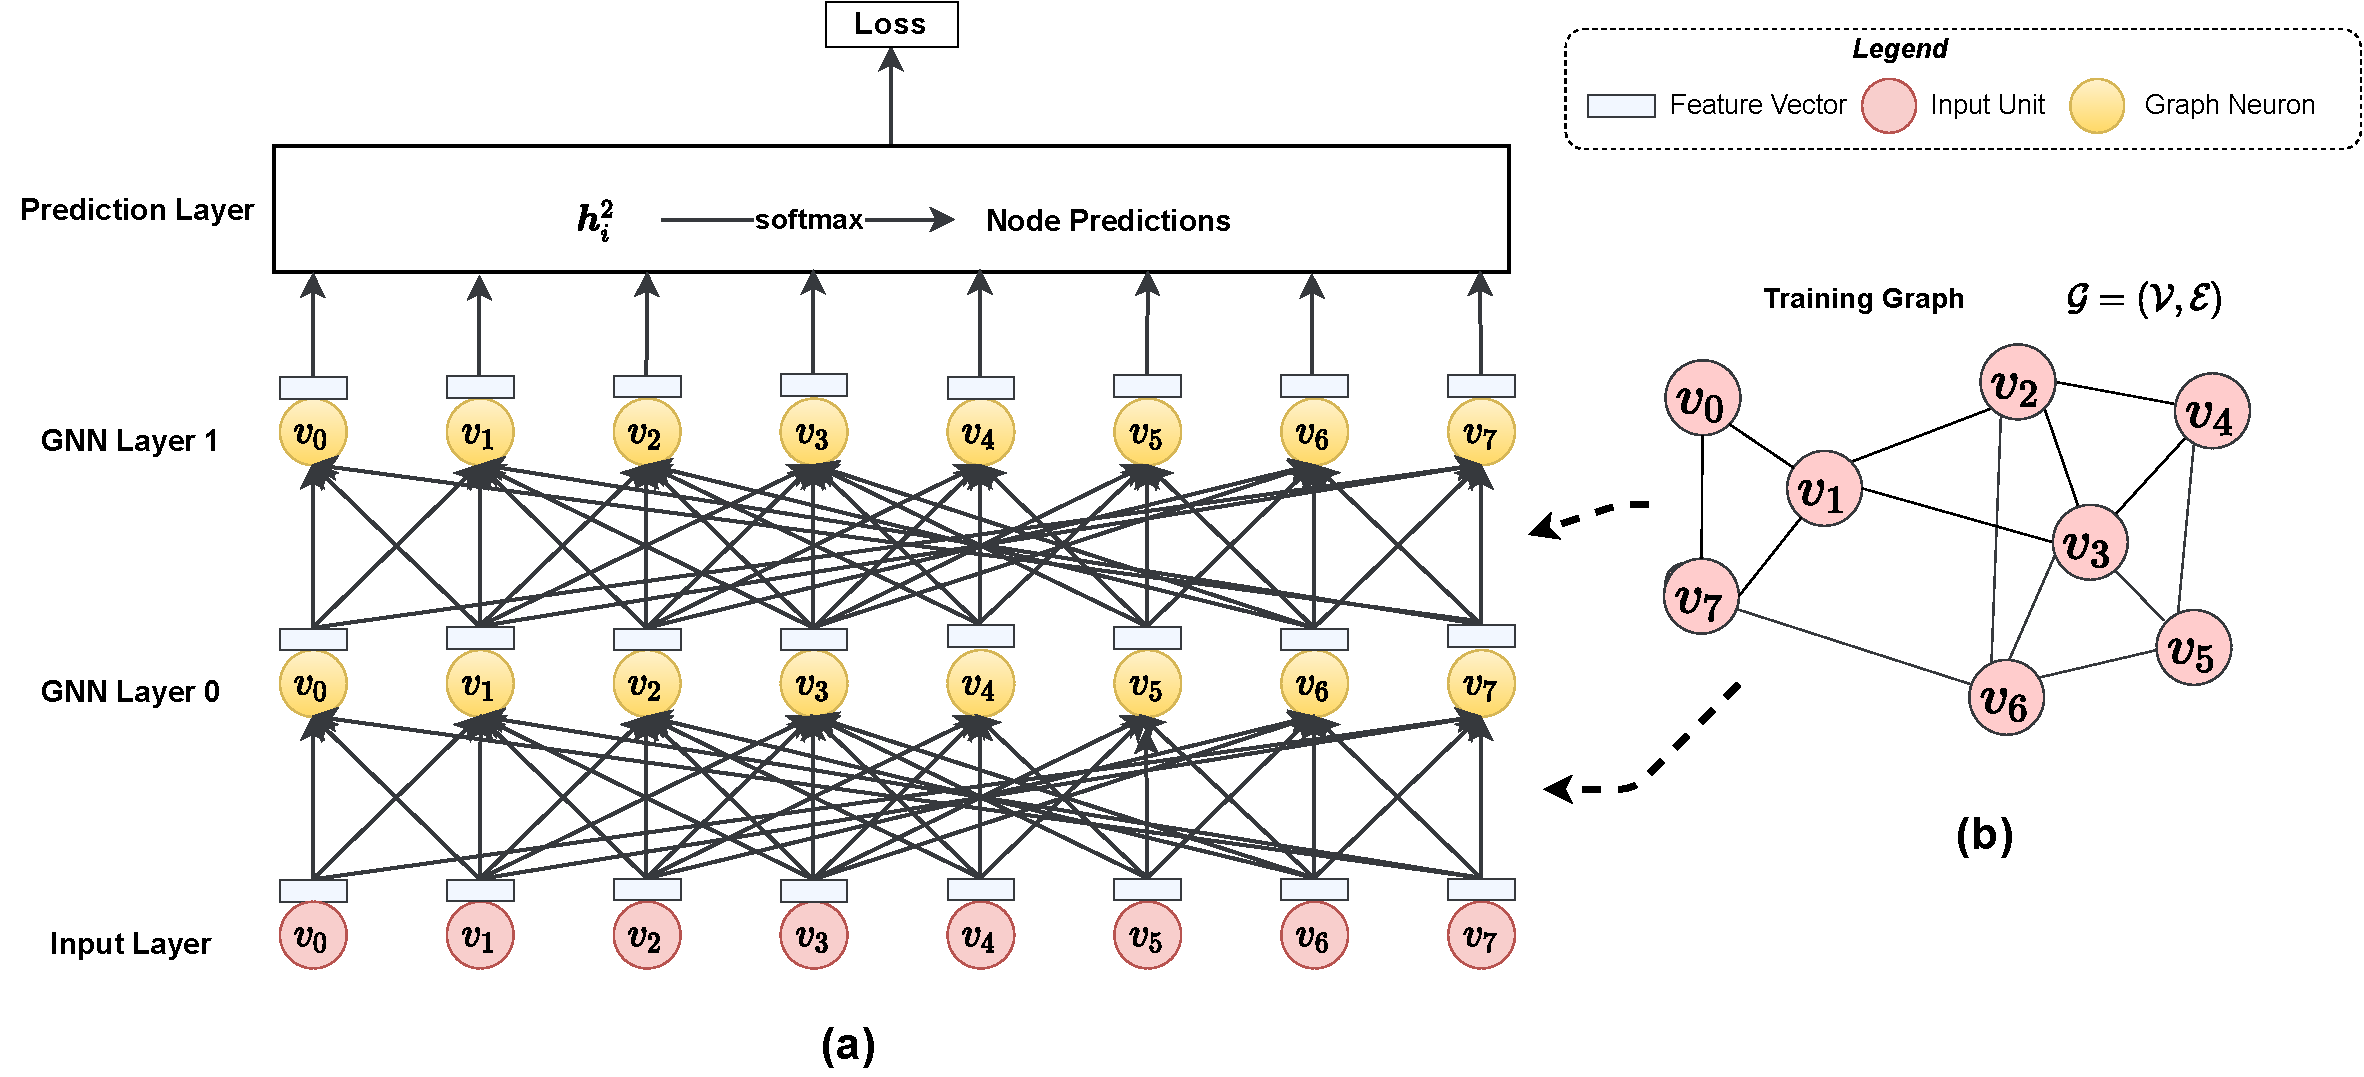
\includegraphics[width=0.95\columnwidth]{figs/illustration/GNN_common_architecture.pdf}
    \caption{Structure of a typical graph neural network. (a) Demo GNN, (b) Demo graph. The target application is the node classification. The demo GNN has two GNN layers.}
    \label{fig:general_structure_of_gnn}
\end{figure}

In the input layer, A GNN receives a graph $\mathcal{G}$ as the input.
%
Every vertex $v_x$ in $\mathcal{G}$ is attached with a feature vector $\boldsymbol{v}_x$ to describe the properties of the vertex.
%
Every edge $e_{y,x}$ of $\mathcal{G}$ may also be attached with a feature vector $\boldsymbol{e}_{y,x}$.
%
The input layer of a GNN receives feature vectors from all vertices and passes the feature vectors to the first GNN layer (i.e. GNN layer 0).

A GNN usually consists of more than one GNN layers.
%
Each GNN layer consists of $|\mathcal{V}|$ graph neurons, where $|\mathcal{V}|$ is the number of vertices in $\mathcal{G}$.
%
Each graph neuron corresponds to a vertex in $\mathcal{G}$.
%
Different GNNs mainly differ in the graph neurons that they use.
%
We elaborate on details of graph neurons later.
%
GNN layers are \emph{sparsely} connected with the input layer and other GNN layers.
%
\begin{itemize}
    \item In the first GNN layer (layer 0), a graph neuron collects feature vectors from the input layer.
    %
    For the graph neuron corresponding to the vertex $v_x$, it collects the feature vector $\boldsymbol{v}_x$ and the feature vectors $\boldsymbol{v}_y$ of the vertices $v_y$ that are adjacent to $v_x$ (i.e.  $v_y \in \mathcal{N}(v_x)$).
    %
    The graph neuron aggregates input feature vectors, apply non-linear transformation, and outputs a hidden vector $\boldsymbol{h}^1_x$ for $v_x$.
    %
    Take the demo GNN in \figurename~\ref{fig:general_structure_of_gnn}(a) as an example.
    %
    Since $\mathcal{N}(v_3) = \{v_1, v_2, v_4, v_5, v_6\}$, the graph neuron of $v_3$ at the GNN layer 0 collects the input feature vectors \{$\boldsymbol{v}_1$, $\boldsymbol{v}_2$, $\boldsymbol{v}_3$, $\boldsymbol{v}_4$, $\boldsymbol{v}_5$, $\boldsymbol{v}_6$\} from the input layer and outputs $\boldsymbol{h}^1_3$.
    %
    The connections between the first GNN layer and the input layer  are determined by the topology of $\mathcal{G}$.
    %
    The graph neuron of $v_x$ in the first GNN layer is connected with the input unit of $v_y$  in the input layer only if there is an edge $e_{y,x}$ between $v_y$ and $v_x$ in $\mathcal{G}$.
    %
    Since most real-world graphs are very \emph{sparse} (i.e. $|\mathcal{E}| \ll |\mathcal{V}|^2$), the connections between the first GNN layer and the input layer are also sparse, different from the traditional neural networks.
    
    \item In the next GNN layer (layer 1), the graph neuron corresponding to $v_x$ collects the hidden vector of itself $\boldsymbol{h}^1_x$ and its adjacent vertices ($\boldsymbol{h}^1_y$ with $v_y \in \mathcal{N}(v_x)$) from the \emph{previous} GNN layer.
    %
    Thus, the connections between the first and the second GNN layers are also determined by the topology of $\mathcal{G}$.
    %
    Based on the collected hidden vectors, the graph neuron in the layer 1 outputs a new hidden vector $\boldsymbol{h}^2_x$ for $v_x$.
   
    \item   A GNN allows stacking more GNN layers to support deeper graph analysis.
    %
    Assume there are $L$ GNN layers in total.
    %
    The last GNN layer (layer $L-1$) outputs a hidden vector $\boldsymbol{h}^{L}_x$ for every vertex $v_x$.
    %
    $\boldsymbol{h}^L_x$ is an embedding vector that encodes the knowledge learned from the input layer and all the previous GNN layers.
    %
    Since $\boldsymbol{h}^L_x$ is affected by $v_x$ and the vertices in the $L$-hop neighborhood of $v_x$, analyzing a graph with more GNN layers means analyzing each vertex with a \emph{wider} scope.
    %
    The hidden vectors $\boldsymbol{h}^L_x$ of the last GNN layer are fed to the prediction layer to generate the output for the whole GNN.
\end{itemize}

The prediction layer is a standard neural network.
%
The structure of the prediction layer depends on the prediction task of the GNN.
%
Take the node classification task in \figurename~\ref{fig:general_structure_of_gnn} as the example.
%
The node classification predicts a label for every vertex in $\mathcal{G}$.
%
In this case, the prediction layer can be a simple softmax layer with $\boldsymbol{h}^L_x$ as the input and a vector of probabilities as the output.
%
If the prediction task is the edge prediction, the hidden vectors of two vertices are concatenated and fed into a softmax layer.
%
If we need to predict a label for the whole graph, a pooling (max/mean/...) layer is added to generate an embedding vector for the whole graph and the embedding vector is used to produce the final prediction.

Supporting end-to-end training is a prominent advantage of GNNs, compared with traditional graph-based machine learning methods.
The traditional methods need to construct input feature vectors for vertices and edges manually or use embedding methods like DeepWalk \cite{bryan2014_deepwalk} and node2vec \cite{aditya2016_node2vec}.
The feature vector generation is independent from the model training.
Therefore, generated feature vectors may not be suitable for downstream prediction tasks.
In GNNs, gradients are propagated from the prediction layer back to GNN layers layer by layer. 
The model parameters in the GNN layers are updated based on the feedbacks from the downstream prediction task. 
In a fully parameterized way, a GNN can automatically extract an embedding vector for each vertex from its $L$-hop neighborhood, tuned according to the specific prediction task.

\subsection{Graph Neuron and Message-passing Model}

Graph neurons are building blocks of a GNN.
%
A GNN layer consists of $|\mathcal{V}|$ graph neurons.
%
Each vertex corresponds to a graph neuron.
%
A graph neuron is a small neural network.
%
For the graph neuron corresponding to $v_x$ at the layer $l$, it receives the hidden vector of itself $\boldsymbol{h}^l_x$ and the hidden vectors of its adjacent vertices $\boldsymbol{h}^l_y$ with $v_y \in \mathcal{N}(v_x)$ from the previous GNN layer\footnote{For the GNN layer 0, graph neurons receive input feature vectors, i.e., $\boldsymbol{h}^0_x=\boldsymbol{v}_x$}.
%
The graph neuron of $v_x$ aggregates the received hidden vectors, applies non-linear transformations, and outputs a new hidden vector $\boldsymbol{h}_x^{l+1}$.

We follow the message-passing model \cite{gilmer_messgae_passing} to formally define a graph neuron.
%
The message-passing model is widely used in the cutting-edge GNN libraries like PyG \cite{PyG} and DGL \cite{DGL}.
%
\figurename~\ref{fig:graph_neuron_structure} shows the internal structure of a graph neuron in the message-passing model.
%
A graph neuron at the layer $l$ are made of three \emph{differentiable} functions: the messaging function $\phi^l$, the aggregation function $\Sigma^l$, and the updating function $\gamma^l$.

\begin{figure}[h]
    \centering
    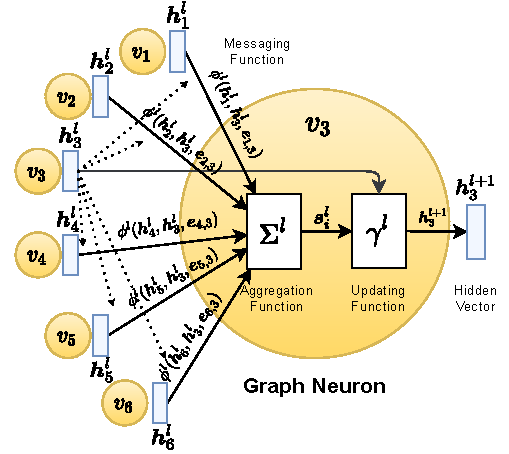
\includegraphics[width=0.5\columnwidth]{figs/illustration/GNN_Unit.pdf}
    \caption{Graph neuron of $v_3$ in the GNN layer $l$ with the demo graph $\mathcal{G}$ in \figurename~\ref{fig:general_structure_of_gnn}b. $\phi^l$/$\Sigma^l$/$\gamma^l$ are the messaging/aggregation/updating functions in the message-passing model, respecitvely.}
    \label{fig:graph_neuron_structure}
\end{figure}

The graph neuron of $v_x$ calculates the output hidden vector $\boldsymbol{h}^{l+1}_x$ with the three functions in three steps:
%
\begin{enumerate}
    %
    \item  For every adjacent edge $(v_y, v_x)$ of $v_x$ ($v_y \in \mathcal{N}(v_x)$), the messaging function $\phi^l$ receives the output hidden vectors $\boldsymbol{h}^l_x$ and $\boldsymbol{h}^l_y$ from the previous GNN layer and the edge feature vector $\boldsymbol{e}_{y,x}$ (and other feature vectors associated with $v_x$/$v_y$ if necessary) as the input.
    %
    $\phi^l$ emits a \emph{message vector} $\boldsymbol{m}^l_{y,x}$ for every edge $(v_y, v_x)$ at the layer $l$, i.e. $\boldsymbol{m}^l_{y,x} = \phi^l(\boldsymbol{h}^l_y, \boldsymbol{h}^l_x, \boldsymbol{e}_{y,x}, \dots)$;
    %
    \item The aggregation function $\Sigma^l$ then aggregates the message vectors $\boldsymbol{m}^l_{y,x}$ of the adjacent edges ($v_y \in \mathcal{N}(v_x)$) to produce an \emph{aggregated vector} $\boldsymbol{s}^l_x$, i.e. $\boldsymbol{s}^l_{x} = \sum^l_{v_y \in \mathcal{N}(v_x)}{\boldsymbol{m}^l_{y,x}}$;
    %
    \item The updating function $\gamma^l$ calculates the {hidden vector} of this layer $\boldsymbol{h}^{l+1}_x$ based on the hidden vector from the previous layer $\MyVec{h}^l_x$ and the aggregated vector $\MyVec{s}^l_x$ (and other feature vectors associated with $v_x$ if necessary), i.e. $\boldsymbol{h}^{l+1}_x = \gamma^l(\boldsymbol{h}^l_x, \boldsymbol{s}^l_x, \dots)$.
\end{enumerate}

Briefly, the behaviour of a graph neuron under the message-passing model can be defined as  

\begin{equation}
      \MyVec{h}^{l+1}_x = \gamma^l(\MyVec{h}^l_x, \mathlarger{\Sigma}^l_{v_y \in \MyVec{N}(v_x)}{\phi^l(\MyVec{h}^l_y, \MyVec{h}^l_x,   \MyVec{e}_{y,x}, \dots)}, \dots).
\end{equation}

%The three functions are small neural networks and parameterized with trainable weight vectors or matrices.
The end-to-end training requires $\phi^l$ and $\gamma^l$ (like multi-layer perceptrons and GRUs) and $\Sigma^l$ (like mean, sum, element-wise min/max) are \emph{differentiable} to make the whole GNN differentiable.

Different GNNs have different definitions of the three functions.
%
We regard $\phi$ and $\Sigma$ as \emph{edge calculation} functions, since they are conducted over every edge in $\mathcal{G}$.
%
We regard $\gamma$ as the \emph{vertex calculation} function, as it is conducted over every vertex in $\mathcal{G}$.
%
\tablename~\ref{tab:gnn_overview_edge} and \tablename~\ref{tab:gnn_overview_vertex} list the edge calculation functions and the vertex calculation functions of typical GNNs, respectively.
%
Some complex GNNs like GAT \cite{huang2018_gat} and GaAN  \cite{zhang2018_gaan} use more than one message passing phase in each GNN layer.
%
We regard every message passing phase in a GNN layer as a \emph{sub-layer}.
%
We will give out more details on sub-layers when we introduce GAT.

%For ChebNet, we report its GNN sub-layer in the tables.
%A ChebNet layer consists of $K$ GNN sub-layers and a summation layer:
%$\boldsymbol{H}^{l+1} = \sum_{k=1}^K{\boldsymbol{Z}^{(k)} \textcolor{blue}{\boldsymbol{W}^{(k)}}}$ with the GNN sub-layers $\boldsymbol{Z}^{(1)}=\boldsymbol{H}^l$, %$\boldsymbol{Z}^{(2)}=\hat{\boldsymbol{L}}\boldsymbol{H}^l$, and $\boldsymbol{Z}^{(k)}=2\hat{\boldsymbol{L}}\boldsymbol{Z}^{(k-1)} - \boldsymbol{Z}^{(k-2)}$, where $\boldsymbol{H}^l$ is the matrix of output hidden feature vectors of the layer $l-1$.
%For GAT, a GAT layer consists of two sub-layers and it conducts part of the vertex calculation before the two sub-layers.
%For GaAN, a GaAN layer consists of four sub-layers: the first sub-layer calculates the summation $\boldsymbol{m}_{j, i, (k)}^{l,0}  = \exp((\textcolor{blue}{W^{l, k}_{xa}} \boldsymbol{h}_j^l + \textcolor{blue}{b^{l, k}_{xa}})^T (\textcolor{blue}{\boldsymbol{W}^{l, k}_{ya}} \boldsymbol{h}_i^l + \textcolor{blue}{\boldsymbol{b}^{l,k}_{ya}}))$, and the other three sub-layers calculate $\boldsymbol{m}^l_{j,i,1}$/$\boldsymbol{m}^l_{j,i,2}$/$\boldsymbol{m}^l_{j,i,3}$.

\newcommand{\GATCalcWeight}{\exp(LeakyReLU(\Param{\MyVec{a}}^T[\hvec{y}[k] \parallel \hvec{x}[k]]))}

\begin{table}[H]
    \hspace{-2em}
    \begin{footnotesize}
        \begin{tabular}{cccp{22em}r}
            \toprule
            GNN                                                                                                                       &
            Type                                                                                                                      &
            $\Sigma^l$                                                                                                                  &
            $\phi^l(\MyVec{h}^{l}_y, \MyVec{h}^l_x, \MyVec{e}_{y,x}, \dots)$                                                                                                                    &
            Complexity                                                                                                                  \\ \midrule
            ChebNet \cite{defferrad2016_chebnet}                                                                                      &
            Spectral                                                                                                                  &
            sum                                                                                                                       &
            $\boldsymbol{m}_{y, x}^{l} = \MyVec{e}_{y, x}\boldsymbol{h}^{l}_y$                                                          &
            $O(d_{in})$                                                                                                   \\
            \textbf{GCN} \cite{kipf2017_gcn}                                                                                          &
            Spectral                                                                                                                  &
            sum                                                                                                                       &
            $\boldsymbol{m}^l_{y, x} = \MyVec{e}_{y, x} \boldsymbol{h}^l_y$                                                                   &
            $O(d_{in})$                                                                                                                 \\
            AGCN \cite{li2018_agcn}                                                                                                   &
            Spectral                                                                                                                  &
            sum                                                                                                                       &
            $\boldsymbol{m}^l_{y, x} = \tilde{e}^l_{y, x} \boldsymbol{h}^l_y$                                                         &
            $O(d_{in})$                                                                                                                 \\
            GraphSAGE \cite{hamilton2017_graphsage}                                                                                   &
            Non-spectral                                                                                                              &
            mean/LSTM                                                                                                                 &
            $\boldsymbol{m}_{y, x}^l =  \boldsymbol{h}_y^l$                                                                           &
            $O(1)$                                                                                                                      \\
            GraphSAGE-pool \cite{hamilton2017_graphsage}                                                                              &
            Non-spectral                                                                                                              &
            max                                                                                                                       &
            $\MyVec{m}_{y, x}^l =  \delta(\Param{\MyMat{W}^l_{pool}} \MyVec{h}_y^l + \Param{b^l})$ &
            $O(d_{in} * d_{out})$                                                                                                       \\
            Neural FPs  \cite{duvenaud2015_neural_fps}                                                                                &
            Non-spectral                                                                                                              &
            sum                                                                                                                       &
            $\boldsymbol{m}_{y, x}^l = \boldsymbol{h}_y^l$                                                                            &
            $O(1)$                                                                                                                      \\
            SSE \cite{han2018_sse}                                                                                                    &
            Recurrent                                                                                                                 &
            sum                                                                                                                       &
            $\boldsymbol{m}_{y, x}^l = \MyVec{v}_y \parallel \boldsymbol{h}_y^l$                                               &
            $O(f+d_{in})$                                                                                                               \\
            \textbf{GGNN}  \cite{li2015_ggnn}                                                                                         &
            Gated                                                                                                                     &
            sum                                                                                                                       &
            $\MyVec{m}^l_{y, x} = \MyVec{\hat{h}}^l_y$                                           &
            $O(d_{in} * d_{out})$                                                                                                       \\
            \textbf{GAT}   \cite{huang2018_gat}                                                                                       &
            Attention                                                                                                                 &
            sum                                                                                                                       &
            \begin{scriptsize}
                $\begin{aligned}[t]
                         & \text{Sub-layer 0:}                                                                                                                                                                                    \\
                         & \MyVec{m}^{l,0}_{y,x}  = \parallel_{k=1}^{K}\GATCalcWeight                                    \\
                         & \text{Sub-layer 1 (multi-head concatenation):}                                                                                                                                                                                    \\
                         & \MyVec{m}^{l,1}_{y,x} = \parallel_{k=1}^{K}\frac{\GATCalcWeight}{\MyVec{h}^{l,0}_x[k]}\hvec{y}[k] \\
                         & \text{Sub-layer 1 (multi-head average)}: \\
                         & \boldsymbol{m}_{j, i}^{l,1} = \frac{1}{K}\sum_{k=1}^K \frac{\GATCalcWeight}{\MyVec{h}^{l,0}_x[k]}\hvec{y}[k]                                                         \\
                    \end{aligned}$
            \end{scriptsize}
                                                                                                                                      &
            $
                \begin{aligned}[t]
                    \text{concat: } O(d_{out})      & \\
                    \text{average: } O(K * d_{out}) & \\
                    \text{Two Sub-layers}           &
                \end{aligned}
            $
            \\
            \textbf{GaAN}     \cite{zhang2018_gaan}                                                                                   &
            Attention                                                                                                                 &
            \begin{scriptsize}\makecell[t]{Sub-layer 0: \\sum\\ Sub-layer 1:\\sum\\Sub-layer 2:\\max\\Sub-layer 3:\\mean}\end{scriptsize}                                                                                                              &
            \begin{scriptsize}
                $\begin{aligned}[t]
                         & \text{Sub-layer 0:}                                                                                                                                                                                                                                                                  \\
                         & \boldsymbol{m}_{y, x}^{l,0}  =\parallel_{k=1}^K \exp((\Param{\MyMat{W}^{l}_{(k), 1}}\MyVec{h}_y^l + \Param{\MyVec{b}^{l}_{(k),1}})^T (\Param{\MyMat{W}^{l}_{(k), 2}}\MyVec{h}_x^l + \Param{\MyVec{b}^{l}_{(k),2}}))                                   \\
%                         & \boldsymbol{m}_{j, i, (k)}^{l,0}  =\parallel_{k=1}^K \exp((\textcolor{blue}{W^{l, k}_{xa}} \boldsymbol{h}_j^l + \textcolor{blue}{b^{l, k}_{xa}})^T (\textcolor{blue}{\boldsymbol{W}^{l, k}_{ya}} \boldsymbol{h}_i^l + \textcolor{blue}{\boldsymbol{b}^{l,k}_{ya}}))                                   \\
                         & \text{Sub-layer 1:}                                                                                                                                                                                                                                                                  \\
                         & \alpha_{(k)} = \frac {\exp((\Param{\MyMat{W}^{l}_{(k), 1}}\MyVec{h}_y^l + \Param{\MyVec{b}^{l}_{(k),1}})^T (\Param{\MyMat{W}^{l}_{(k), 2}}\MyVec{h}_x^l + \Param{\MyVec{b}^{l}_{(k),2}}))} {\MyVec{h}^{l,0}_{x}[k]} \\
                         & \boldsymbol{m}_{y, x}^{l, 1} = \parallel_{k=1}^K \alpha_{(k)} LeakyReLU(\Param{\boldsymbol{W}^{l}_{(k),v}} \MyVec{h}_y^l + \Param{\MyVec{b}^{l}_{(k),v}})                                                                                                           \\
                         & \text{Sub-layer 2:}                                                                                                                                                                                                                                                                  \\
                         & \boldsymbol{m}_{y, x}^{l, 2} = \Param{\MyMat{W}^l_m} \MyVec{h}_y^{l} + \Param{\MyVec{b}^l_m}                                                                                                                                                      \\
                         & \text{Sub-layer 3:}                                                                                                                                                                                                                                                                  \\
                         & \boldsymbol{m}_{y, x}^{l, 3} = \MyVec{h}_y^l
                    \end{aligned}$
            \end{scriptsize}                                                                                            &
            \makecell[tr]{$O(\max(d_a, d_v, d_m) * K * d_{in})$                                                                           \\
                Four Sub-layers \\ 
                $\Param{\MyMat{W}^l_{(k),1}} \in \mathbb{R}^{d_a \times d_{in}}$ \\
                $\Param{\MyMat{W}^l_{(k),v}} \in \mathbb{R}^{d_v \times d_{in}}$ \\
                $\Param{\MyMat{W}^l_{m}} \in \mathbb{R}^{d_m \times d_{in}}$ 
            }                                                                                                            \\
            \bottomrule
        \end{tabular}
    \end{footnotesize}
    \caption{Typical graph neural networks and their edge calculation functions.
        $d_{in}$ and $d_{out}$ are the dimensions of the input and output hidden vectors, respectively.
        Blue variables are model parameters to learn.
        $\delta$ is the activation function.
    }
    \label{tab:gnn_overview_edge}
\end{table}

\begin{table}[H]
    \centering
    \begin{footnotesize}
        \begin{tabular}{clr}
            \toprule
            GNN                                                                                                                                                                                                              &
            $\gamma^l(\boldsymbol{h}^l_x, \boldsymbol{s}^l_x, \dots)$                                                                                                                                                                                                         &
            Complexity                                                                                                                                                                                                         \\ \midrule
            ChebNet \cite{defferrad2016_chebnet}                                                                                                                                                                             &
            $\MyVec{h}_x^{l+1} = 2\boldsymbol{s}^{l}_{x} - \boldsymbol{h}_x^{l-1}$                                                                                                                                  &
            $O(d_{out})$                                                                                                                                                                                                       \\
            \textbf{GCN} \cite{kipf2017_gcn}                                                                                                                                                                                 &
            $\boldsymbol{h}_x^{l+1} = \textcolor{blue}{\boldsymbol{W}}^l  \boldsymbol{s}_x^{l}$                                                                                                                              &
            $O(d_{in} * d_{out})$                                                                                                                                                                                              \\
            AGCN   \cite{li2018_agcn}                                                                                                                                                                                        &
            $\boldsymbol{h}_x^{l+1} = \textcolor{blue}{\boldsymbol{W}}^l  \boldsymbol{s}_x^{l}$                                                                                                                              &
            $O(d_{in} * d_{out})$                                                                                                                                                                                              \\
            GraphSAGE  \cite{hamilton2017_graphsage}                                                                                                                                                                         &
            $\boldsymbol{h}_x^{l+1} =   \delta(\textcolor{blue}{\boldsymbol{W}}^l  [\boldsymbol{s}_x^{l} \parallel \boldsymbol{h}_x^l])$                                                                                     &
            $O(d_{in} * d_{out})$                                                                                                                                                                                              \\
            GraphSAGE-pool   \cite{hamilton2017_graphsage}                                                                                                                                                                   &
            $\boldsymbol{h}_x^{l+1} = \boldsymbol{s}_x^l$                                                                                                                                                                    &
            $O(1)$                                                                                                                                                                                                             \\
            Neural FPs        \cite{duvenaud2015_neural_fps}                                                                                                                                                                 &
            $\boldsymbol{h}_x^{l+1} = \delta(\textcolor{blue}{\boldsymbol{W}}^{l, |\mathcal{N}(v_i)|}  (\boldsymbol{h}_x^l + \boldsymbol{s}_x^{l}))$                                                                           &
            $O(d_{in} * d_{out})$                                                                                                                                                                                              \\
            SSE             \cite{han2018_sse}                                                                                                                                                                               &
            $\boldsymbol{h}_x^{l+1} = (1 - \alpha)  \boldsymbol{h}_x^l +\alpha    \delta(\textcolor{blue}{\boldsymbol{W}}^l_1 \delta(\textcolor{blue}{\boldsymbol{W}}^l_2 [\boldsymbol{v}_x \parallel \boldsymbol{s}_x^l]))$ &
            $O((f + d_{in}) * d_{out})$                                                                                                                                                                                        \\
            \textbf{GGNN}    \cite{li2015_ggnn}                                                                                                                                                                              &
            \begin{scriptsize}
                $\begin{aligned}[t]
                         & \text{Preprocessing: } \MyVec{\hat{h}}^l_x = \Param {\MyMat{W}^l}\boldsymbol{h}^l_x; \\
                         & {\boldsymbol{z}}_x^l = \delta ( \textcolor{blue}{\boldsymbol{W}^z} \boldsymbol{s}_x^l + \textcolor{blue}{\boldsymbol{b}^{sz}} + \textcolor{blue}{\boldsymbol{U}^z} \boldsymbol{h}_x^{l} + \textcolor{blue}{\boldsymbol{b}^{hz}})                    \\
                         & \boldsymbol{r}_x^l = \delta ( \textcolor{blue}{\boldsymbol{W}^r} \boldsymbol{s}_x^l+ \textcolor{blue}{\boldsymbol{b}^{sr}} +\textcolor{blue}{\boldsymbol{U}^r} \boldsymbol{h}_x^{l} + \textcolor{blue}{\boldsymbol{b}^{hr}})                        \\
                         & \boldsymbol{\bar{h}}_x^{l+1} = \tanh ( \textcolor{blue}{\boldsymbol{W}} \boldsymbol{s}_x^l + \textcolor{blue}{\boldsymbol{b}^s} + \textcolor{blue}{\boldsymbol{U}} ( \boldsymbol{r}_x^l \odot \boldsymbol{h}_x^{l}) + \textcolor{blue}{\boldsymbol{b}^h}) \\
                         & \boldsymbol{h}_x^{l+1} = (1 - {\boldsymbol{z}}_x^l) \odot \boldsymbol{h}_x^l + {\boldsymbol{z}}_x^l \odot \boldsymbol{\bar{h}}_x^{l+1}
                    \end{aligned}$
            \end{scriptsize}
                                                                                                                                                                                                                             &
            $O(d_{in} * d_{out})$                                                                                                                                                                                              \\
            \textbf{GAT} \cite{huang2018_gat}                                                                                                                                                                                &
            \begin{scriptsize}
                $\begin{aligned}[t]
                         & \text{Preprocessing: } \hat{\boldsymbol{h}}^{l}_{x} = \parallel_{k=1}^K \Param{\MyMat{W}^l_{(k)}}\MyVec{h}^l_x;        \\
                         & \text{Sub-layer 0:}                                                                            \\
                         & \MyVec{h}^{l,0}_{x} = \MyVec{s}^{l,0}_{x}                              \\
                         & \text{Sub-layer 1:}                                                                            \\
                         & \boldsymbol{h}_x^{l+1} = \MyVec{h}^{l,1}_x = \delta(\boldsymbol{s}_x^{l,1})
                    \end{aligned}
                $
            \end{scriptsize}                                                                                                                                                                                   &
            $
                \begin{aligned}[t]
                    \text{concat:} O(d_{in}*d_{out})    & \\
                    \text{average:} O(K*d_{in}*d_{out}) & \\
                    \text{Two Sub-layers}               &
                \end{aligned}
            $
            \\
            \textbf{GaAN}  \cite{zhang2018_gaan}                                                                                                                                                               &
            \begin{scriptsize}
                $\begin{aligned}[t]
                         & \text{Sub-layer 0/1/2:}                                                                                                                                                                            \\
                         & \MyVec{h}^{l,*}_{x} = \MyVec{s}^{l,*}_{x}                                                                                                                              \\
                         & \text{Sub-layer 3:}                                                                                                                                                                      \\
                         & \boldsymbol{g}_x^l = \textcolor{blue}{\boldsymbol{W}^l_g}[\boldsymbol{h}_x^{l} \parallel \boldsymbol{h}_{x}^{l, 2} \parallel \boldsymbol{s}_{x}^{l, 3}] + \textcolor{blue}{\boldsymbol{b}^l_g} \\
                         & \boldsymbol{h}_x^{l+1} = \MyVec{h}^{l,3}_x = \textcolor{blue}{\boldsymbol{W}^l_o} [\boldsymbol{h}_x^l \parallel (\boldsymbol{g}_{x}^l \odot \boldsymbol{h}_{x}^{l, 1})] + \textcolor{blue}{\boldsymbol{b}^l_o}
                    \end{aligned}$
            \end{scriptsize}                                                                                                                                                                                   &
            \makecell[r]{$O(\max(K * d_v + d_{in}$, \\ $2 * d_{in} + d_m) * d_{out})$                                                                                                                                                \\
                Four Sub-layers}
            \\ \bottomrule
        \end{tabular}
    \end{footnotesize}
    \caption{Typical graph neural networks and their vertex calculation functions.
        $d_{in}$ and $d_{out}$ are the dimensions of the input and output hidden vectors, respectively.
        Blue variables are model parameters to learn.
        In Neural FPs, $\textcolor{blue}{\boldsymbol{W}}^{l, |\mathcal{N}(i)|}$ is the weight matrix for vertices with degree $|\mathcal{N}(i)|$ at the layer $l$.
        $\delta$ is the activation function.
    }
    \label{tab:gnn_overview_vertex}
\end{table}

\subsection{Representative GNNs}

%Since we focus on analyzing the performance bottleneck in training GNNs, we classify the typical GNNs from the view of time complexity.
We use $O_\phi$/$O_\Sigma$/$O_\gamma$ to denote the time complexity of the three functions in the message-passing model.
The time complexity of a GNN layer is made up of two parts: the edge calculation complexity $O_\phi$ + $O_\Sigma$ and the vertex calculation complexity $O_\gamma$.
%
In \tablename~\ref{tab:gnn_overview_edge} and \tablename~\ref{tab:gnn_overview_vertex}, we list the edge and vertex calculation complexity of each GNN, respectively.
The time complexity of a graph neuron is affected by the dimensions of the input/output hidden vectors $d_{in}$ and $d_{out}$ and the dimensions of the model parameters (like the number of heads $K$ in GAT and the dimensions of the view vectors $d_a$/$d_v$/$d_m$ in GaAN).

Since we focus on analyzing the performance bottleneck in training GNNs, we classify the typical GNNs into four quadrants based on their edge/vertex complexity as shown in \figurename~\ref{fig:gnn_complexity_quadrant}. We pick GCN, GGNN, GAT, and GaAN as the \emph{representative} GNNs of the four quadrants.

\begin{figure}[h]
    \centering
    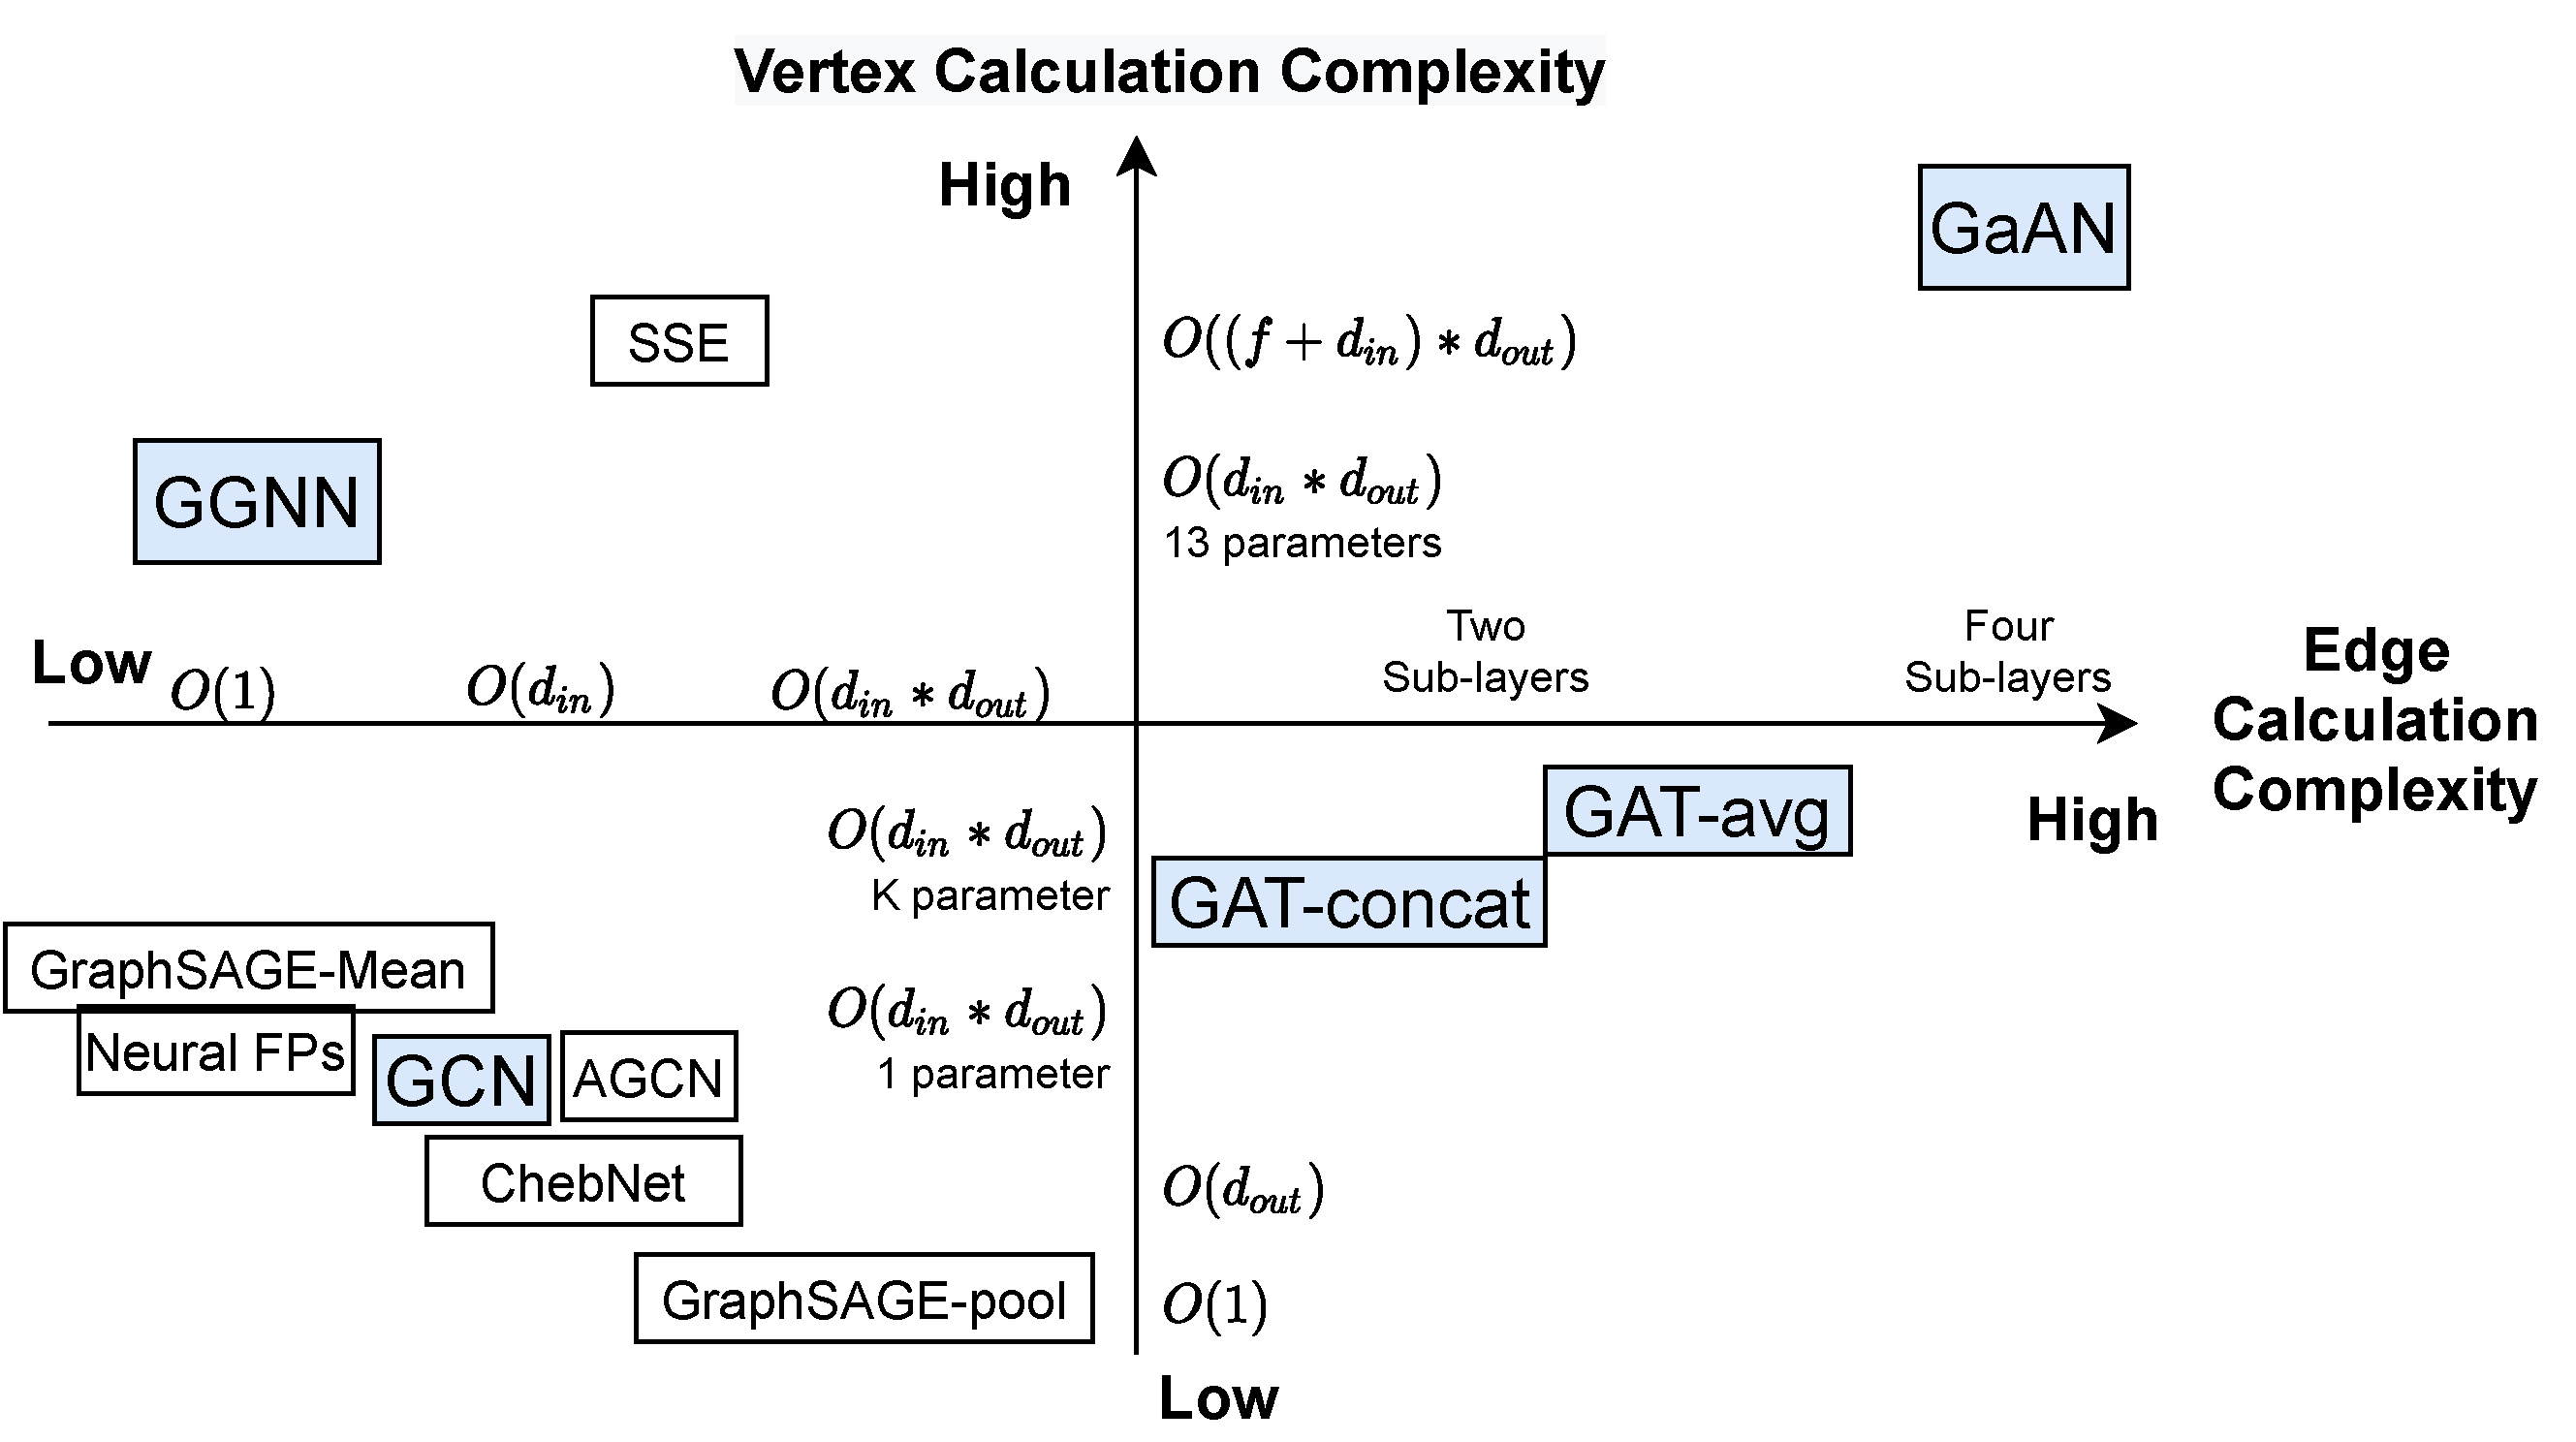
\includegraphics[width=0.8\columnwidth]{figs/illustration/GNN_complexity_quadrant.pdf}
    \caption{Complexity quadrants of typical GNNs. We compare the complexity according to the number of sub-layers, the Big-O notation, and the number of parameters to train.}
    \label{fig:gnn_complexity_quadrant}
\end{figure}

\subsubsection{GCN (Low Vertex \& Low Edge Complexity)}

Graph convolution network (GCN \cite{kipf2017_gcn}) introduces the first-order approximation of the spectral-based graph convolutions into graph neural networks.
%
It has only one parameter to learn at each layer, i.e. the weight matrix $\Param{\MyMat{W}^l}$ in the updating function $\gamma^l$.
%
A GCN graph neuron can be expressed as $\boldsymbol{h}^{l+1}_x = \Param{\MyMat{W}^l}\sum_{v_y \in \mathcal{N}(v_x)}{w_{y,x}\boldsymbol{h}^l_y}$, where $w_{y,x}$ is the normalized weight of the edge $e_{y,x}$.
%
According to the associative law of the matrix multiplication, $\boldsymbol{h}^{l+1}_x = \sum_{v_y \in \mathcal{N}(v_x)}{w_{y,x}\Param{\MyMat{W}^l}\boldsymbol{h}^l_y}$.
%
Since the dimension of $\boldsymbol{h}^{l+1}_x$ is usually smaller than $\boldsymbol{h}^l_x$ in practical GCNs, the implementation of GCN in PyG chooses to first conduct the vertex calculation $\hat{\boldsymbol{h}}^l_y = \Param{\MyMat{W}^l}\boldsymbol{h}^l_y$ for each vertex $v_y$ and then conduct the edge calculation $\boldsymbol{h}^{l+1}_x=\sum_{v_y\in\mathcal{N}(v_x)}{w_{y,x}\hat{\boldsymbol{h}}^l_y}$.
%
As $\hat{\boldsymbol{h}}^l_y$ has the same dimension as $\boldsymbol{h}^{l+1}_x$, the implementation significantly reduces the  computation cost of the edge calculation.

\subsubsection{GGNN (High Vertex \& Low Edge Complexity)}

GGNN \cite{li2015_ggnn} introduces the gated recurrent unit (GRU) into graph neural networks.
%
The updating function $\phi^l$ of GGNN is a modified GRU unit that has 12 model parameters to learn, having high computational complexity.
%
To lower the training cost, all GNN layers share the same group of parameters in GGNN.
%
GGNN further requires the dimension of $\boldsymbol{h}^{l+1}$ is equal to the dimension of $\boldsymbol{h}^l$.
%
Since the messaging function $\phi^l$ only uses the hidden vector $\boldsymbol{h}^l_y$ of the source vertex $v_y$ for an edge $e_{y,x}$, in the implementation of PyG, GGNN conducts the pre-processing vertex calculation $\MyVec{\hat{h}}^l_x = \Param {\MyMat{W}^l}\boldsymbol{h}^l_x$ for every vertex $v_x$ before the message passing.
%
The messaging function $\phi^l$ directly uses $\MyVec{\hat{h}}^l_y$ as the message vector for every edge $e_{y, x}$.
%
In this way, GGNN further reduces the time complexity of the edge calculation to $O(1)$ without increasing the time complexity of the vertex calculation.

\subsubsection{GAT (Low Vertex \& High Edge Complexity)}

GAT \cite{huang2018_gat} introduces the multi-head attention mechanism into graph neural networks.
%
Each GAT layer has $K$ heads that generate $K$ independent views for an edge, where $K$ is a hyper-parameter.
%
The views of $K$ heads can be merged by concatenating or by averaging.
%
For concatenating, the dimension of the hidden vector of each head $d_{head}$ is $d_{out}/K$.
%
For averaging, $d_{head}$ is $d_{out}$.

Each GAT layer consists of a vertex pre-processing phase and two sub-layers (i.e., message-passing phases).

The vertex pre-processing phase calculates the attention vector $\hat{\boldsymbol{h}}^{l}_{x}$ for every vertex $v_x$ by $\hvec{x} = \parallel_{k=1}^K \Param{\MyMat{W}^l_{(k)}}\MyVec{h}^l_x$. We denote the attention sub-vector generated by the $k$-th head as $\hvec{x}[k]=\Param{\MyMat{W}^l_{(k)}}\MyVec{h}^l_x$.

The first sub-layer of GAT (defined in Equation~\ref{eq:GAT-sub-layer-1}) uses the attention vectors to emit the attention weight vector $\boldsymbol{m}^{l,0}_{y,x}$ for every edge $e_{y,x}$ and aggregates the attention weight vectors for every vertex $v_x$ to get the weight sum vector $\MyVec{h}^{l,0}_x$.
%
\begin{equation}
    \label{eq:GAT-sub-layer-1}
    \begin{aligned}
        \MyVec{m}^{l,0}_{y,x} & = \phi^{l,0}(\MyVec{h}^l_y, \MyVec{h}^l_x, \MyVec{e}_{y,x}, \hvec{y}, \hvec{x}) = \parallel_{k=1}^{K}\GATCalcWeight, \\
        \MyVec{s}^{l,0}_{x} &= \mathlarger{\Sigma}_{v_y \in \mathcal{N}(v_x)}{\MyVec{m}^{l,0}_{y,x}}, \\
        \MyVec{h}^{l,0}_{x} &= \gamma^{l,0}(\MyVec{h}^l_x, \MyVec{s}^{l,0}_{x})  = \MyVec{s}^{l,0}_{x}.
    \end{aligned}
\end{equation}
%
The second sub-layer of GAT (defined in Equation~\ref{eq:GAT-sub-layer-2}) uses the weight sum vectors to normalize the attention weights for every edge and aggregates the attention vectors $\boldsymbol{\hat{h}}^l_y$ with the normalized weights.
%
The aggregated attention vectors $\MyVec{s}^{l,1}_x$ are transformed by an activation function $\delta$ and are outputted as the hidden vectors of the current layer $\MyVec{h}^{l+1}_x$.
%
\begin{equation}
        \label{eq:GAT-sub-layer-2}
    \begin{aligned}
        \MyVec{m}^{l,1}_{y,x} &= \phi^{l,1}(\MyVec{h}^{l,0}_y, \MyVec{h}^{l,0}_x, \MyVec{e}_{y,x}, \hvec{y}, \hvec{x}) = \parallel_{k=1}^{K}\frac{\GATCalcWeight}{\MyVec{h}^{l,0}_x[k]}\hvec{y}[k], \\
        \MyVec{s}^{l,1}_x &= \mathlarger{\Sigma}_{v_y \in \mathcal{N}(v_x)} \MyVec{m}^{l,1}_{y,x}, \\
        \MyVec{h}^{l+1}_x = \MyVec{h}^{l,1}_x &= \gamma^{l,1}(\MyVec{h}^{l,0}, \MyVec{s}^{l,1}_x) = \delta(\MyVec{s}^{l,1}_x).
    \end{aligned}
\end{equation}

\subsubsection{GaAN (High Vertex \& High Edge Complexity)}

Based on the multi-head mechanism, GaAN \cite{zhang2018_gaan} introduces a convolutional subnetwork to control the weight of each head.
%
Each GaAN layer consists of four sub-layers (as defined in Table~\ref{tab:gnn_overview_edge} and Table~\ref{tab:gnn_overview_vertex}).
%
The first two sub-layers are similar to GAT, and the last two sub-layers build the convolutional subnetwork.
%
The first sub-layer aims to get the sum of attention weights of every vertex in all heads $\MyVec{h}^{l,0}_x$.
The second sub-layer aggregates the hidden vectors from the previous GaAN layer with the normalized attention weights for all heads $\alpha_{(k)}$.
The third and fourth sub-layers aggregate the hidden vectors from the GaAN previous layer with the element-wise max and mean operators separately.
The vertex updating funciton $\gamma^{l,3}$ of the fourth sub-layer uses the hidden vectors of the last two sub-layers $\MyVec{h}^{l, 1}_x, \MyVec{h}^{l, 2}_x$ to generate the output hidden vector $\MyVec{h}^{l+1}_x$.

\subsection{Sampling Techniques}

By default, GNNs are trained in a full-batch way, using the whole graph in each iteration.
%
But the full-batch gradient descent has two disadvantages \cite{chiang2019_cluster_gcn}:
%
(1) it has to cache intermediate results of all vertices in the forward phase, consuming lots of memory space, which is not scalable;
%
(2) it updates the model parameters only once for each epoch, slowing the convergence of gradient descent.

To train GNNs in a mini-batch way, the sampling techniques \cite{hamilton2017_graphsage, ying2018_pinsage, chen2018_fastgcn, chen2018_sgcn, zeng2018_aesg, chiang2019_cluster_gcn, zeng2020_graphsaint} are proposed.
%
In each mini-batch, they sample a small subgraph from the whole graph $\mathcal{G}$ and uses the subgraph to update the model parameters.
%
The sampling techniques only active the graph neurons and the connections that appear in the sampled subgraph between GNN layers, as shown in \figurename~\ref{fig:gnn_sampling}.
%
Inactive graph neurons and connections do not participate in the training of this mini-batch, saving lots of computation and storage costs.
%
Moreover, it may reduce the risk of overfitting the training graph.
%
The existing sampling techniques can be classified into two groups: \emph{neighbor sampling} and \emph{graph sampling}, based on whether different GNN layers sample different subgraphs.

The neighbor sampling techniques \cite{hamilton2017_graphsage, ying2018_pinsage, chen2018_fastgcn, chen2018_sgcn, huang2018_adap} sample nodes or edges layer by layer.
%
The sampled subgraphs of different GNN layers may be \emph{different}, as shown in \figurename~\ref{fig:gnn_sampling}(a).
%
GraphSAGE \cite{hamilton2017_graphsage} is a representative neighbor sampling technique.
%
The tecnnique first samples several vertices from $\mathcal{V}$ in the last GNN layer.
%
Then it repeatedly samples the neighbors of the sampled vertices from the previous layer until the input layer.
%
For every sampled vertex $v_x$ in the GNN layer $l$, GraphSAGE samples at most $\eta^l$ neighbors of $v_x$ from the previous layer.
%
$\eta^l$ is the hyper-parameter that is usually much smaller than $|\mathcal{V}|$.
%
By this way, GraphSAGE limits neighborhood sizes of vertices in the sampled subgraph, especially high-degree vertices.

\begin{figure}[H]
    \centering
    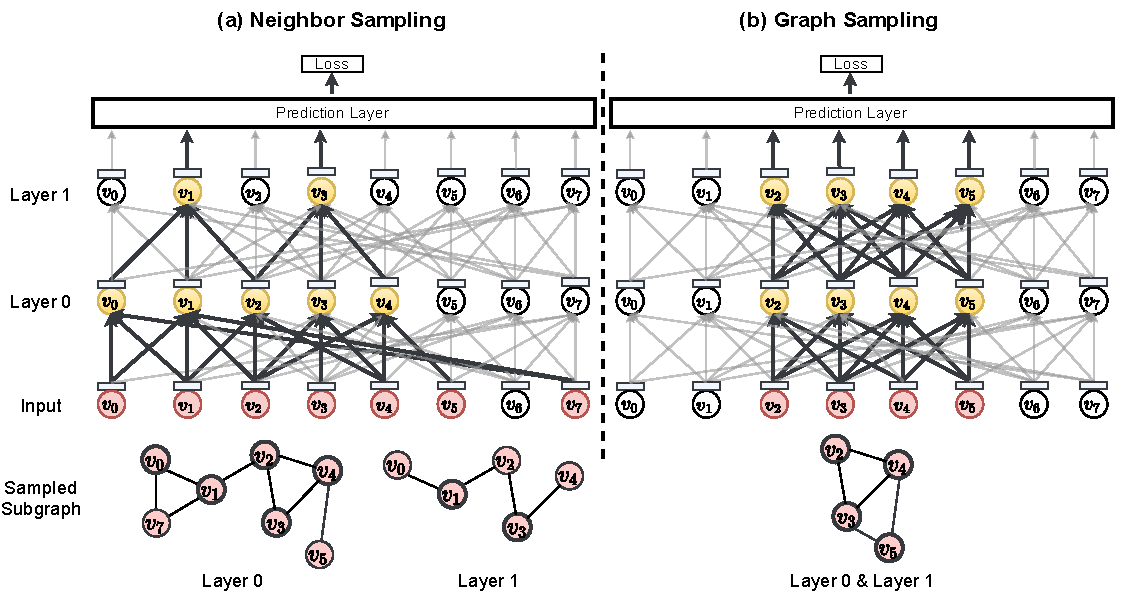
\includegraphics[width=0.9\columnwidth]{figs/illustration/sampling_techniques.pdf}
    %\subfloat[Neighbor sampling\label{fig:gnn_sampling_neighbor_sampling}]{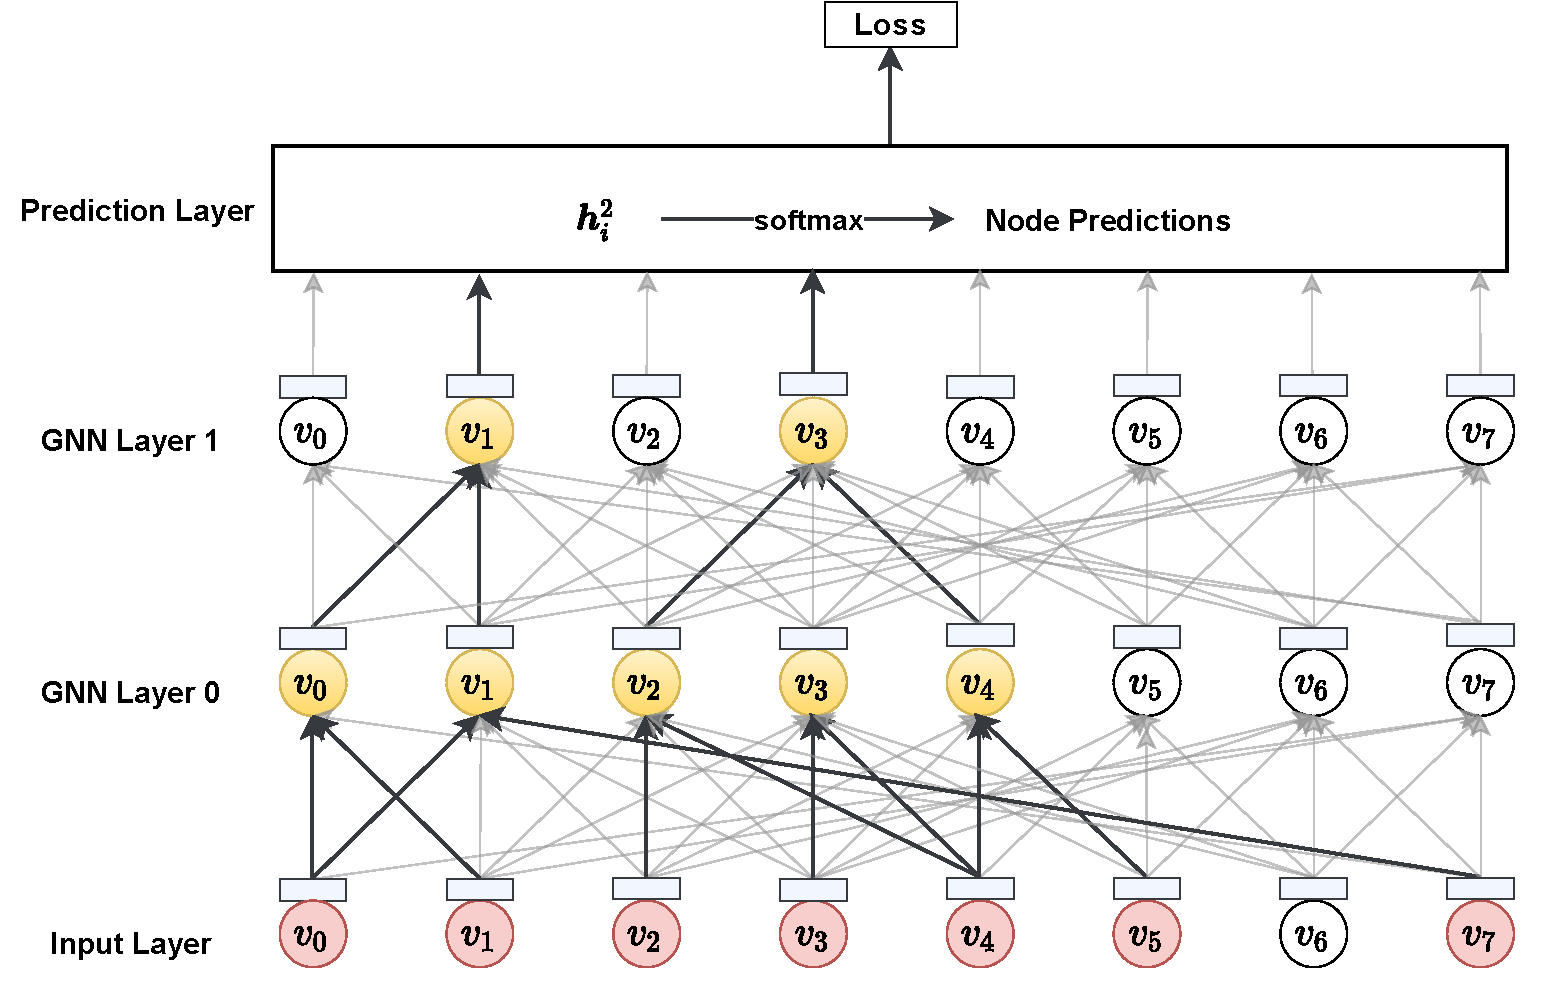
\includegraphics[height=4.5cm]{figs/illustration/layer_sampling.pdf}}
    %
    %\subfloat[Graph sampling\label{fig:gnn_sampling_graph_sampling}]{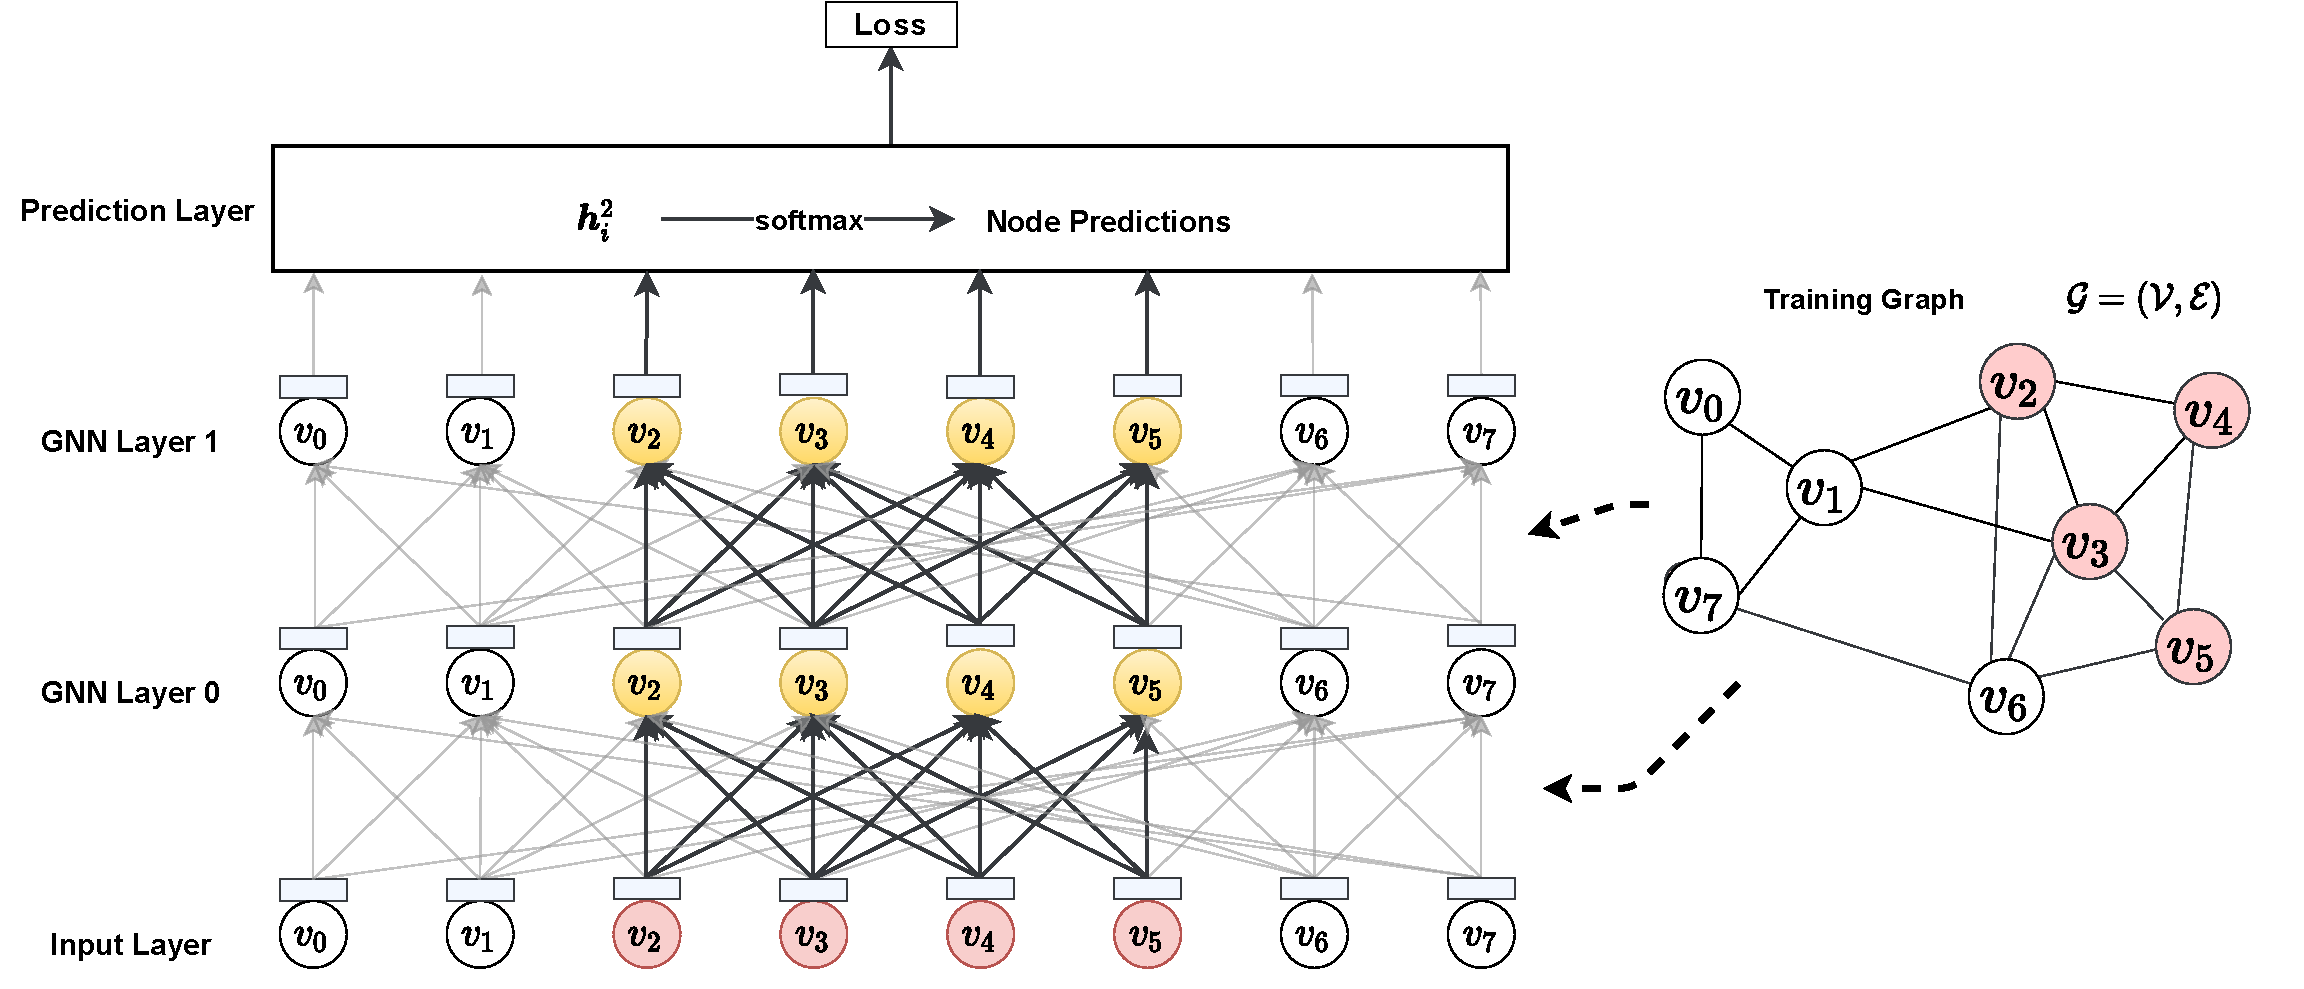
\includegraphics[height=4.5cm]{figs/illustration/graph_sampling.pdf}}
    \caption{Training a GNN with sampling techniques. The faded graph neurons and their connections are inactivated.}
    \label{fig:gnn_sampling}
\end{figure}

The graph sampling techniques \cite{zeng2018_aesg, chiang2019_cluster_gcn, zeng2020_graphsaint} sample a subgraph for each mini-batch and use the same sampled subgraph for all GNN layers, as shown in \figurename~\ref{fig:gnn_sampling}(b).
%
They differ in how to sample subgraphs.
%
The cluster sampler technique \cite{chiang2019_cluster_gcn} is a representative graph sampling technique.
%
Given a training graph $\mathcal{G}$, it partitions $\mathcal{G}$ into several dense clusters.
%
For each mini-batch, it randomly pick $N$ clusters to form the sampled subgraph, where $N$ is the hyper-parameter.

In the implementation in PyG, the model parameters of GNNs reside on the GPU side and the input graph resides on the host side.
%
To process an epoch, PyG samples the original graph in the main memory and generates several batches for the epoch.
%
For each batch, PyG sends the sampled subgraph to the GPU, propagates the feature vectors of the sampled subgraph from the input layer to the prediction layer, calculates the gradients on the subgraph, and updates the model parameters based on the gradients directly on the GPU.
%
With the sampling techniques, the model parameters are updated by a stochastic gradient descent optimizer.
%
PyG conducts the evaluation phase every several epochs or batches (either on the CPU side or the GPU side) to determine whether to stop the training.


\subsection{Inference with GNNs}

The model parameters of a GNN are stored in the weight vectors/matrices of the prediction layer and the messaging/aggregation/updating functions of each GNN layer.
%
When we want to perform inference on a new graph based on a trained GNN, the structure of the GNN needs to be adjusted, but the hyper-parameters and the model parameters of the GNN remain unchanged.
%
The number of graph neurons in each GNN layer has to be adjusted to $|\mathcal{V}|$ of the new graph.
%
The connections of graph neurons between GNN layers also needs to be adjusted according to the edge set of the new graph.

During inference, input feature vectors of the new graph are propagated forward from the input layer to the prediction layer to give out predicted labels.
%
The workflow of inference is the same as the workflow of the \emph{forward} phase during training.
%
The only difference from the forward phase is that there is no need to cache intermediate calculation results during inference, because inference does not need to prepare for gradient calculation.

Inference methods can be divided into two types based on the range of input graphs involved in inference: full-batch inference and sample-based inference.
%
The full-batch inference performs inference on the whole input graph at once.
%
It can make full use of the computing power of GPUs, bringing high computation efficiency.
%
The full-batch inference is suitable for small graphs that the GPU memory can hold all feature vectors, models, and intermediate results.

Different from the full-batch inference, the sample-based inference only predicts labels for part of vertices/edges each time, limiting the GPU memory usage during inference.
%
It first samples a subgraph related to inference from the input graph and then performs the full-batch inference on the sampled subgraph.
%
The sampling method depends on the prediction task.
%
Taking the node classification scenario as an example, if there are $L$ GNN layers in the GNN, the hidden vector outputted by the last GNN layer of each vertex $\MyVec{h}^L_x$ is only related to the $L$-hop neighborhood of $v_x$.
%
Thus, if we want to predict labels for a group of vertices, we only need to sample a subgraph that contains $L$-hop neighborhoods of all given vertices.
%
The sample-based inference is suitable for processing big graphs.
%
It stores the whole input graph and its feature vectors in the main memory.
%
It processes the whole graph in batches.
%
The subgraph of each batch is sampled on the CPU side and sent to the GPU side to perform inference.
%
By using small batch sizes, the peak memory usage during inference can be limited under the GPU memory capacity.
%
The sample-based inference is also suitable for the online inference scenario that the topology of the graph evolves over time.
%
When a graph update arrives, the subgraph affected by the update is sampled and inferences are only performed on the sampled subgraph.it. that are affected by , avoiding conducting repeated inferences for the whole graph.

